\subsection{扩张的张量积}

命题 1. --- 设 \(\Omega\) 是域 \(K\) 的一个扩张，并令 \(L, M\) 为 \(\Omega\) 的两个在 \(K\) 上代数不相交的子扩张。假设 \(K\) 在 \(L\) 中的相对可分代数闭包等于 \(K^1\) 。设 \(\varphi\) 为 \(L \otimes_K M\) 到 \(\Omega\) 中的 K-代数同态，它把 \(x \otimes y\) 映为 \(xy\) （对于 \(x \in L\) , \(y \in M\) ），并设 \(\mathfrak{p}\) 是 \(\varphi\) 的核，则 \(\mathfrak{p}\) 是 \(L \otimes_K M\) 的幂零元集合，且它是 \(L \otimes_K M\) 的最小素理想。

必要时将 \(\Omega\) 替换为一个代数闭包，我们可以假设 \(\Omega\) 是代数闭的。设 B 为 M 在 K 上的一个超越基，N 为 \(\mathrm{K}(\mathrm{B})\) 在 \(\Omega\) 中的相对代数闭包， \(\mathrm{N}_{s}\) （相应地 \(N_{r}\) ）为 N 的在 \(\mathrm{K}(\mathrm{B})\) 上可分（相应地，p-根式）的元素集合。我们注意到 M 在 \(\mathrm{K}(\mathrm{B})\) 上是代数的，因此 N 是 M 在 \(\Omega\) 中的相对代数闭包。

\pandocbounded{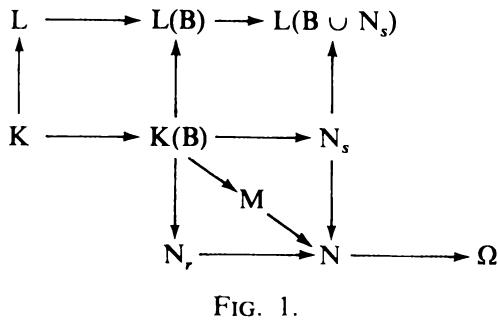
\includegraphics[keepaspectratio]{images/part002_5eeda79f.jpg}}

让我们定义以下同态链：

\[
\begin{array}{r l} & {\mathrm{L} \otimes_ {\mathrm{K}} \mathrm{M} \xrightarrow {\alpha} \mathrm{L} \otimes_ {\mathrm{K}} \mathrm{N} \xrightarrow {\beta} (\mathrm{L} \otimes_ {\mathrm{K}} \mathrm{K} (\mathrm{B})) \otimes_ {\mathrm{K} (\mathrm{B})} \mathrm{N} \xrightarrow {\gamma} \mathrm{L} (\mathrm{B}) \otimes_ {\mathrm{K} (\mathrm{B})} \mathrm{N}} \\ & {\xrightarrow {\delta} \mathrm{L} (\mathrm{B}) \otimes_ {\mathrm{K} (\mathrm{B})} \mathrm{N}_s \otimes_ {\mathrm{K} (\mathrm{B})} \mathrm{N}_r \xrightarrow {\varepsilon} \mathrm{L} (\mathrm{B} \cup \mathrm{N}_s) \otimes_ {\mathrm{K} (\mathrm{B})} \mathrm{N}_r \xrightarrow {\zeta} \Omega .} \end{array}
\]

我们有 \(\alpha = \mathrm{Id}_{\mathbf{L}} \otimes u\) ，其中 \(u\) 是 M 到 N 中的典范嵌入，因此 \(\alpha\) 是单射。映射 \(\beta\) 是交换群的同构，它把 \(x \otimes y\) 映为 \((x \otimes 1) \otimes y\) （II，第 278 页，命题 2），对于 \(x \in L\) 和 \(y \in N\) 。我们有 \(\gamma = v \otimes \mathrm{Id}_{\mathbf{N}}\) ，其中 \(v\) 是 \(\mathrm{L} \otimes_{\mathbf{K}} \mathrm{K}(\mathrm{B})\) 到 \(\mathrm{L}(\mathrm{B})\) 中的、把 \(x \otimes y\) 映为 \(xy\) 的 K-代数同态（对于 \(x \in L\) 和 \(y \in \mathrm{K}(\mathrm{B})\) ）；由于 L 和 M 在 K 上代数不相交，命题 14（V，第 114 页）表明 L 和 K(B) 在 K 上线性不相交，换言之， \(v\) 是单射，因此 \(\gamma\) 是单射。由于 N 是 K(B) 的拟伽罗瓦扩张，存在（V，第 76 页，命题 13）一个 K(B)-代数同构 \(w\) ，它把 \(\mathrm{N}_s \otimes_{\mathrm{K}(\mathrm{B})} \mathrm{N}_r\) 同构地映到 N 上，并把 \(x \otimes y\) 映为 \(xy\) （对于 \(x \in \mathbf{N}_s\) 和 \(y \in \mathbf{N}_r\) ）；我们用 \(\delta\) 表示同构 \(\mathrm{Id}_{\mathrm{L(B)}} \otimes w^{-1}\) 。由定理 1（V，第 137 页）以及关于 K 的扩张 L 的假设，L(B) 中每个在 K(B) 上代数且可分的元素都属于 K(B)；特别地，我们有 L(B) \(\cap\) N \(_s\) = K(B)。由于 N \(_s\) 是 K(B) 的伽罗瓦扩张，定理 5（V，第 71 页）表明存在一个 K(B)-代数同构 \(w'\) ，它是 L(B) \(\otimes_{\mathrm{K(B)}} \mathrm{N}_s\) 到 L(B \(\cup\) N \(_s\) ) 上的、把 \(x \otimes y\) 映为 \(xy\) 的映射（对于 \(x \in L(B)\) 和 \(y \in \mathrm{N}_s\) ）；我们用 \(\varepsilon\) 表示同构 \(w' \otimes \mathrm{Id}_{\mathrm{N}_r}\) 。最后， \(\zeta\) 是把 \(x \otimes y\) 映为 \(xy\) 的 K-代数同态（对于 \(x \in L(B \cup \mathrm{N}_s)\) 和 \(y \in \mathrm{N}_r\) ）。

以上所述表明， \(\eta = \varepsilon \delta \gamma \beta \alpha\) 是 \(L \otimes_{K} M\) 到 \(L(B \cup N_s) \otimes_{K(B)} N_r\) 中的单 K-代数同态。进一步地， \(M\) 的每个元素具有形式 \(\sum_{i=1}^{n} a_i b_i\) ，其中 \(a_i \in N_s\) 且 \(b_i \in N_r\) （对于 \(1 \leqslant i \leqslant n\) ）；因此我们得到 \(\varphi = \zeta \eta\) 。

核 \(\mathfrak{p}\) （\(\varphi\) 的）是 \(\mathbf{L} \otimes_{\mathbb{K}} \mathbf{M}\) 的一个素理想，因此由命题 2（V，第 118 页）， \(\mathbf{L} \otimes_{\mathbb{K}} \mathbf{M}\) 的每个幂零元素都属于 \(\mathfrak{p}\) 。反之设 \(a\) 为 \(\mathfrak{p}\) 的一个元素；令 \(\eta(a) = \sum_{i=1}^{s} b_i \otimes c_i\) ，其中 \(b_i \in \mathbf{L}(\mathbf{B} \cup \mathbf{N}_s)\) 且 \(c_i \in \mathbf{N}_r\) （对于 \(1 \leqslant i \leqslant s\) ）。由于

\(N_{r}\) 是 \(K(B)\) 的一个 p-根式扩张，存在一个整数 \(f \geqslant 0\) 使得 \(c_{i}^{p^{f}}\) 属于 \(K(B)\) （对于 \(1 \leqslant i \leqslant s\) ，其中 p 是 K 的特征指数）。但我们有

\[
\eta \left(a ^ {p ^ {f}}\right) = \sum_ {i = 1} ^ {s} b _ {i} ^ {p ^ {f}} \otimes c _ {i} ^ {p ^ {f}} = \left(\sum_ {i = 1} ^ {s} b _ {i} ^ {p ^ {f}} c _ {i} ^ {p ^ {f}}\right) \otimes 1 = \zeta \eta (a) ^ {p ^ {f}} \otimes 1 = 0
\]

且由于 \(\eta\) 是单射，我们最终有 \(a^{p^{f}} = 0\) 。因此我们已证明 \(\mathfrak{p}\) 是 \(\mathrm{L} \otimes_{\mathrm{K}} \mathrm{M}\) 的所有幂零元素的集合。现在，由命题 2（V，第 118 页）， \(\mathrm{L} \otimes_{\mathrm{K}} \mathrm{M}\) 的每个素理想都包含 \(\mathfrak{p}\) 。

推论. --- 设 L 和 M 是域 K 的两个扩域。假设 K 在 L 中的相对可分代数闭包等于 K。则 \(L \otimes_{K} M\) 的幂零元集合 p 是一个素理想。此外，如果 L 或 M 在 K 上是可分的，则 \(L \otimes_{K} M\) 是整环。

我们可以假设 L 和 M 是 K 的某个扩张 \(\Omega\) 的代数不相交的子扩张（V，第 116 页，定理 5）；则根据命题 1（V，第 139 页），p 是素理想。若进一步 L 或 M 在 K 上可分，则由可分扩张的定义（V，第 119 页，定义 1）， \(L \otimes_{K} M\) 是既约环；所以 p = 0 且 \(L \otimes_{K} M\) 是整环，因为 p 原先是素理想。

